\documentclass[tikz]{standalone}
\usetikzlibrary{shapes.geometric,positioning,arrows}
\begin{document}

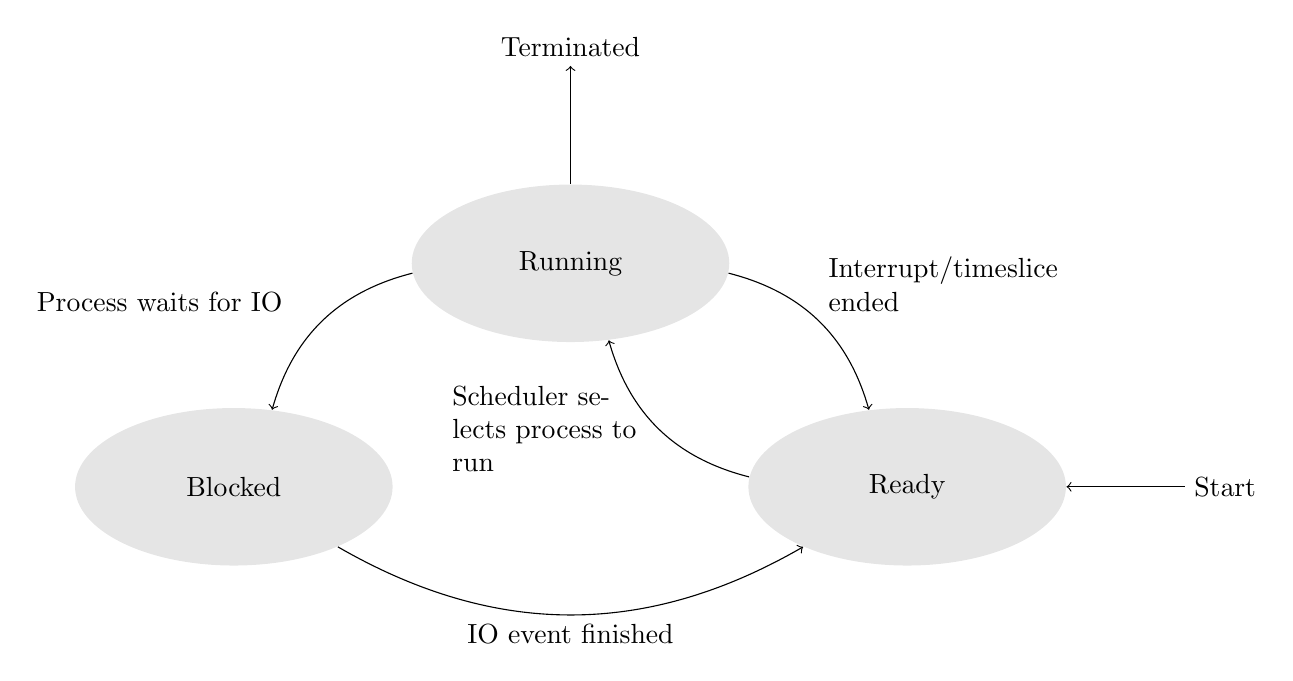
\begin{tikzpicture}[force/.style={},
    ellips/.style={ellipse, minimum width=100pt,
    align=center,node distance=2cm,fill=black!10,inner sep=5pt,text width=2.5cm,minimum 
    height=2.0cm,>=stealth'}
]
  \node[ellips, force] (ready)   {Ready}; 
  \node[force, right=1.5cm of ready] (start)   {Start}; 
  \node[above=2cm of ready](dummy) {}; 
  \node[ellips, force, left=1.5cm of dummy] (running) [above left= of ready] {Running};
  \node[force, above=1.5cm of running] (terminated)   {Terminated}; 
  \node[ellips, force, right=1.5cm of dummy] (blocked) [below left= of running] {Blocked};

  \path[->] (ready)   edge [bend left]  node [anchor=center, text width=2.5cm, left, midway] {Scheduler selects process to run} (running);
  \path[->] (running) edge [bend left]  node [anchor=center, text width=3.5cm, above right, midway] {Interrupt/timeslice ended} (ready);
  \path[->] (running) edge [bend right] node [anchor=center, text width=3.5cm, above left, midway] {Process waits for IO} (blocked);
  \path[->] (blocked) edge [bend right] node [below] {IO event finished} (ready);
  \path[->] (start) edge (ready);
  \path[->] (running) edge (terminated);
\end{tikzpicture}

\end{document}